\documentclass{article}
\usepackage{amssymb} % Required for math symbols
\usepackage{graphicx} % Required for inserting images
\usepackage[hidelinks]{hyperref}
\usepackage{float}

\usepackage[utf8]{inputenc}
\usepackage{amsmath}
\usepackage[a4paper, total={6in, 10in}]{geometry}
\usepackage{listings}
\usepackage{xcolor}

\definecolor{codegray}{rgb}{0.5,0.5,0.5}
\definecolor{codepurple}{rgb}{0.58,0,0.82}
\definecolor{backcolour}{rgb}{0.95,0.95,0.92}

\lstdefinestyle{cppstyle}{
    backgroundcolor=\color{backcolour},   
    commentstyle=\color{codegray}\ttfamily,
    keywordstyle=\color{blue}\bfseries,
    numberstyle=\tiny\color{gray},
    stringstyle=\color{codepurple},
    basicstyle=\ttfamily\footnotesize,
    breaklines=true,
    captionpos=b,
    keepspaces=true,
    numbers=left,
    numbersep=5pt,
    showspaces=false,
    showstringspaces=false,
    showtabs=false,
    tabsize=2,
    language=C++
}

\title{Laboratorio 1 - Arduino}
\author{jeremy.matos@utec.edu.pe, luis.gutierrez@utec.edu.pe}
\date{Abril 2025}

\begin{document}

\maketitle

\newpage
\tableofcontents
\newpage

\section{Introducción}

\subsection{Objetivo General}

\subsection{Objetivos Específicos}

\newpage

\section{Marco teórico}

% TODO: preguntar a que se refiere con la descripcion de los pines

\section{Estado del Arte}

\section{Metodología}

En esta sección se describirá el desarrollo de cada una de las experiencias del laboratorio.

\subsection{Checkpoint 1: Creación de un circuito básico}

Este ejercicio introductorio propone la implementación de un circuito básico utilizando un diodo LED y una resistencia (Figura \ref{fig:circuito_basico}). 
% El objetivo es observar el funcionamiento del diodo LED y medir la caída de tensión en sus terminales.

\begin{figure}[H]
    \centering
    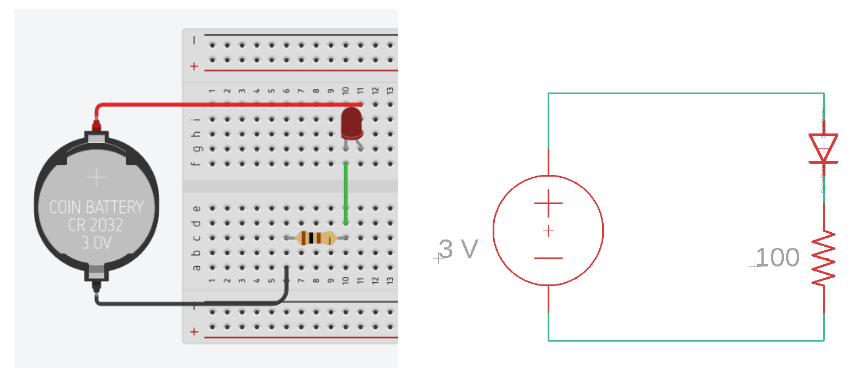
\includegraphics[width=0.85\textwidth]{./img/ckpt_1_0.png}
    \caption{Circuito básico con un diodo LED y una resistencia.}
    \label{fig:circuito_basico}
\end{figure}

\begin{enumerate}
    \item \textbf{Descripción del circuito:} \\
    El circuito está compuesto por una batería tipo moneda de 3V, un diodo LED conectado en serie y una resistencia de 100~$\Omega$ para limitar el paso de corriente. Luego, se conectará un voltímetro en paralelo con el LED para medir la caída de tensión y un amperímetro después de la resistencia para medir la corriente que atraviesa el circuito.

    \item \textbf{¿Cuál es el valor de la caída de tensión en los terminales del diodo LED?} \\
    De acuerdo a la Figura \ref{fig:caida_tension}, la caída de tensión en los terminales del diodo LED es de \textbf{1.98 V}.

    \item \textbf{¿Cuál es el valor de corriente obtenido en el circuito?} \\
    El valor de corriente medido con el amperímetro fue de \textbf{9.30 mA} (miliamperios).

    \item \textbf{¿Cuál es la potencia consumida por el diodo LED?} \\
    Usando la fórmula $P = V \times I$, donde $V = 1.98$ V y $I = 9.3$ mA, se obtiene una potencia de aproximadamente \textbf{18.414 mW}.
\end{enumerate}

\begin{figure}[H]
    \centering
    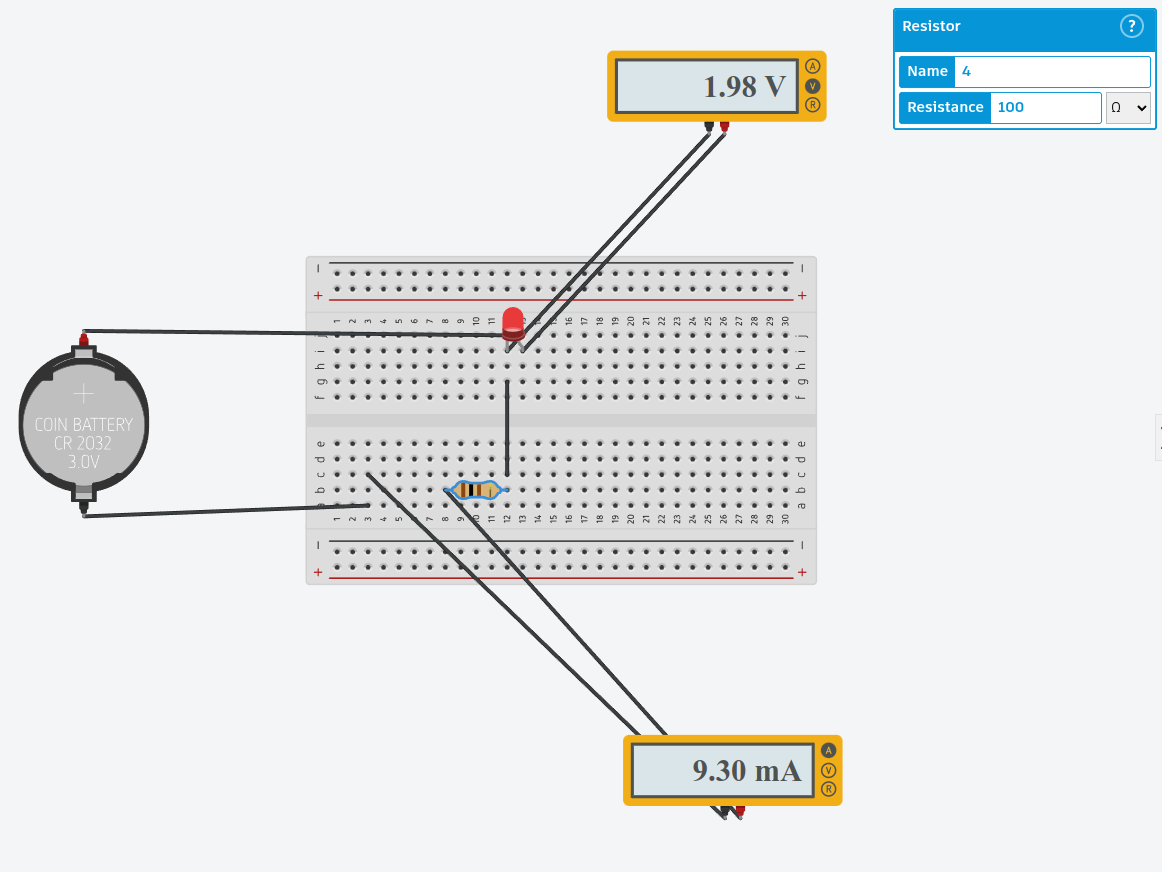
\includegraphics[width=0.85\textwidth]{./img/ckpt_1_1.png}
    \caption{Medida de caída de tensión.}
    \label{fig:caida_tension}
\end{figure}

\subsection{Checkpoint 2: Conexión de resistencias en serie y paralelo}

Similar al ejercicio anterior, se propone la implementación de 2 circuitos con resistencias en serie y paralelo.

\subsubsection{Circuito 1}

El primer circuito consiste en conectar un diodo LED simple a una resistencia como se ve en Figura \ref{fig:resistencia_serie}. Mientras que el segundo propone conectar 2 resistencias en paralelo, como se ve en la Figura \ref{fig:resistencia_paralelo}. 

\begin{figure}[H]
    \centering
    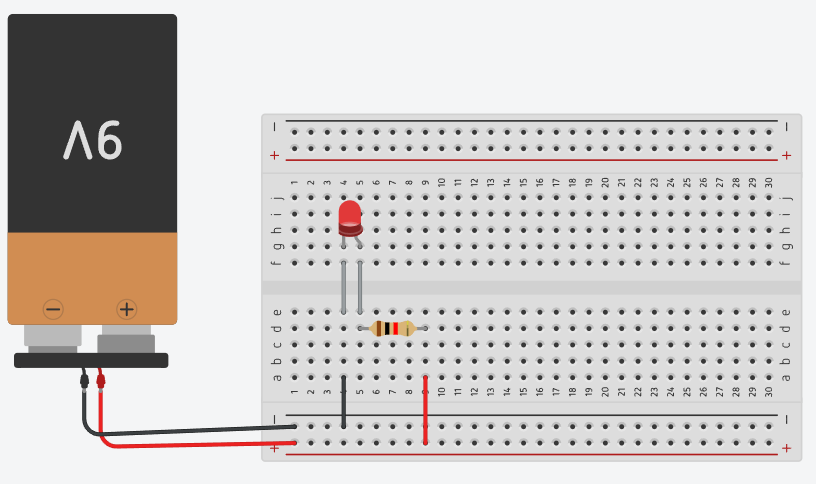
\includegraphics[width=0.5\textwidth]{./img/ckpt_2_1.png}
    \caption{Resistencia en serie}
    \label{fig:resistencia_serie}
\end{figure}


\begin{figure}[H]
    \centering
    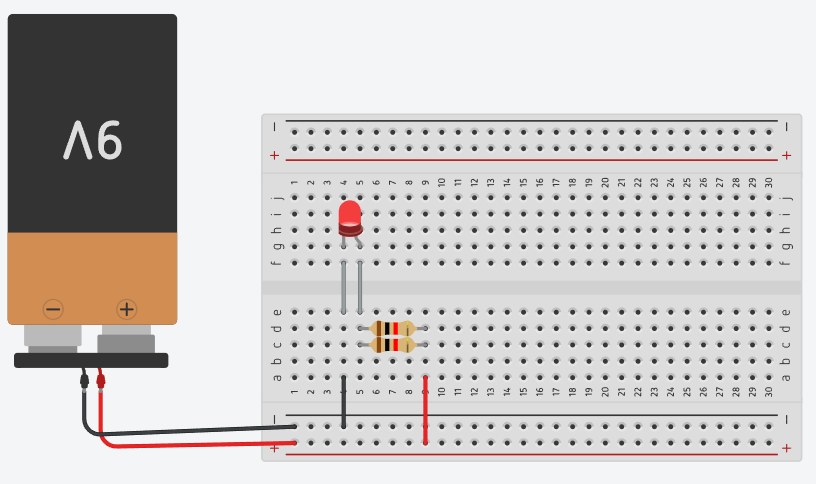
\includegraphics[width=0.5\textwidth]{./img/ckpt_2_2.png}
    \caption{2 Resistencia en paralelo}
    \label{fig:resistencia_paralelo}
\end{figure}

Ambos diodos LED se encienden, ya que las resistencias no limitan suficientemente la corriente que fluye a través de ellos. No obstante, el LED mostrado en la Figura \ref{fig:resistencia_serie} brilla con mayor intensidad en comparación con el de la Figura \ref{fig:resistencia_paralelo}, especialmente si se incrementa el valor de las resistencias.

\subsubsection{Circuito 2}

\begin{figure}[H]
    \centering
    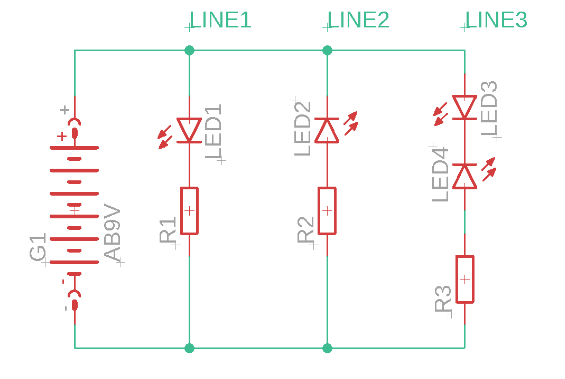
\includegraphics[width=0.5\textwidth]{./img/ckpt_2_3_0.png}
    \caption{Esquema de conexión}
    \label{fig:circuito_2}
\end{figure}

Se solicita simular (Figuras \ref{fig:simulacion_implementacion}, \ref{fig:simulacion_esquema}) en Tinkercad el esquema presentado en la Figura \ref{fig:circuito_2} y responder las siguientes preguntas:

\begin{enumerate}
    \item \textbf{Descripción del circuito:} \\
    El circuito consiste en tres ramas conectadas en paralelo a una fuente de 9V. Cada rama contiene un LED en serie con una resistencia limitadora de corriente. Esto permite que cada LED tenga su propia caída de tensión y que la corriente se divida según la resistencia y características del LED en cada línea.

    \item \textbf{¿Qué sucede con el diodo LED en la Línea 1?} \\
    El LED en la Línea 1 enciende correctamente. La resistencia R1 limita la corriente, permitiendo que el LED funcione dentro de su rango seguro.

    \item \textbf{¿Qué sucede con el diodo LED en la Línea 2?} \\
    El LED en la Línea 2 no enciende. Esto se debe a que la polaridad del diodo está invertida, lo que impide el paso de corriente. En este caso, la resistencia R2 no limita la corriente, ya que el LED no permite que fluya.

    \item \textbf{¿Qué sucede con el diodo LED en la Línea 3? ¿Por qué?} \\
    Ninguno de los LEDs en la Línea 3 enciende. Como ambos están conectados en serie, la caída de tensión total requerida (~4.4V) puede superar la tensión disponible después de la resistencia R3. Además, dado que uno de los LEDs está mal conectado (polaridad invertida), este interrumpe todo el paso de corriente en esa rama, impidiendo que cualquiera de los dos encienda.
\end{enumerate}

\begin{figure}[H]
    \centering
    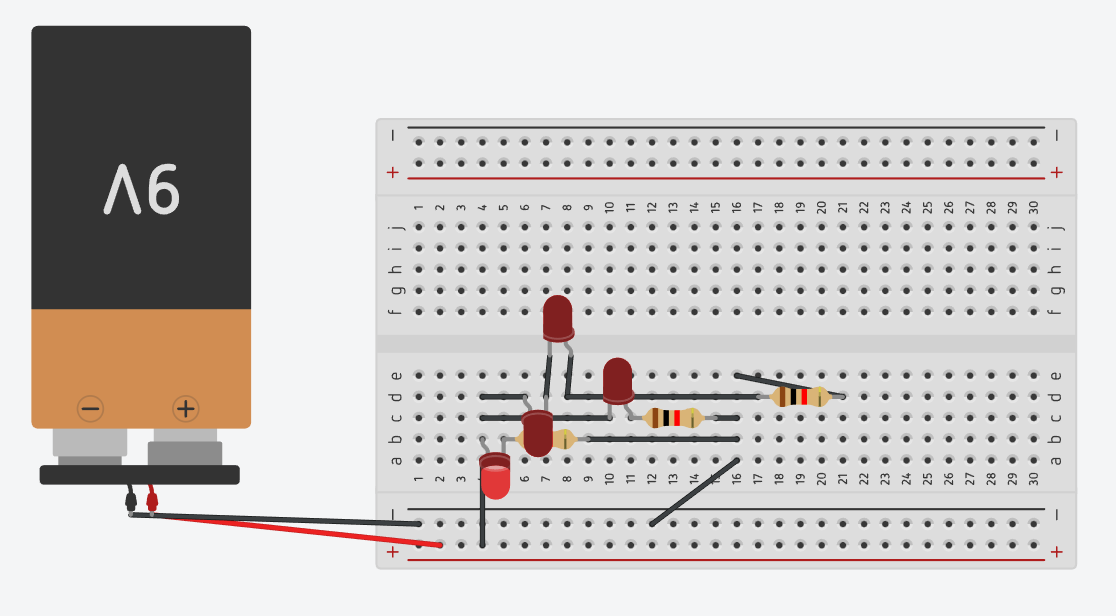
\includegraphics[width=0.85\textwidth]{./img/ckpt_2_3_1.png}
    \caption{Simulación Tinkercad del circuito.}
    \label{fig:simulacion_implementacion}
\end{figure}


\begin{figure}[H]
    \centering
    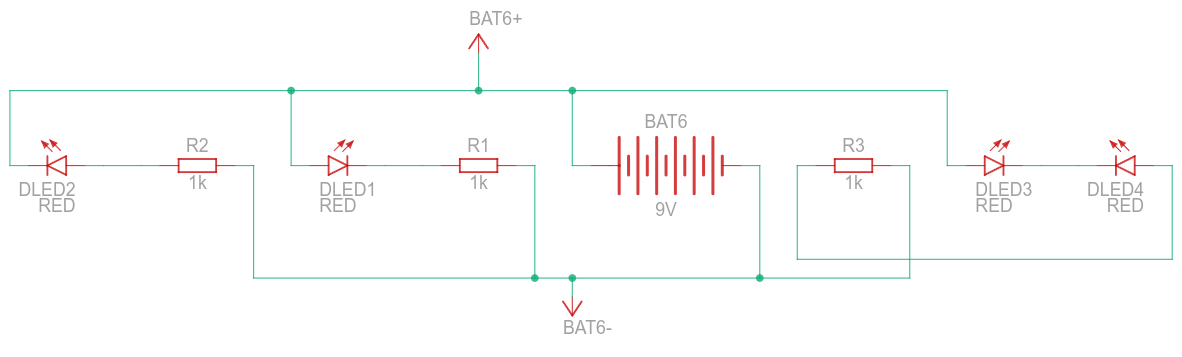
\includegraphics[width=0.85\textwidth]{./img/ckpt_2_3_2.png}
    \caption{Esquema de conexión Tinkercad}
    \label{fig:simulacion_esquema}
\end{figure}

\subsection{Checkpoint 3: Simulación en FALSTAD}
Para el desarrollo de esta parte de la experiencia de laboratorio, nos hemos encargado de construir el siguiente circuito utilizando el programa \textbf{FALSTAD} para su simulacion.

\begin{figure}[H]
    \centering
    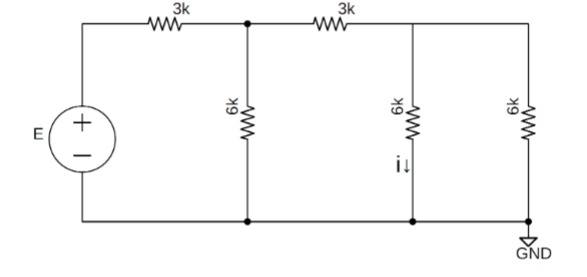
\includegraphics[width=0.85\textwidth]{./img/Circuito-3.jpeg}
    \caption{Circuito base}
    \label{fig:simulacion_esquema}
\end{figure}

\begin{figure}[H]
    \centering
    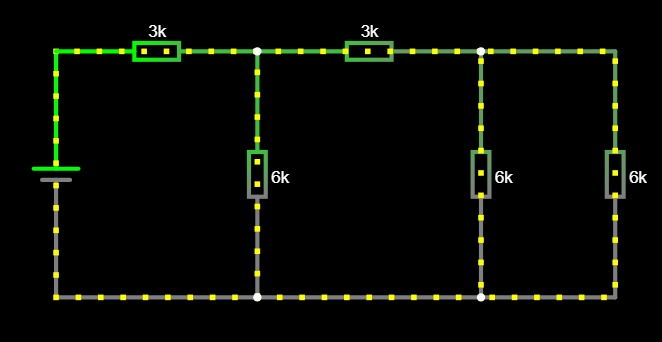
\includegraphics[width=0.85\textwidth]{./img/Falstad.jpeg}
    \caption{Circuito en simulador FALSTAD}
    \label{fig:simulacion_esquema}
\end{figure}

Una vez realizada la simulación, hemos rescatado los siguientes datos:
\begin{itemize}
    \item El valor de la corriente ``i" es de 208.333 $\mu$A
    \item La caída de tensión en la resistencia, siendo la ultima ubicada en la derecha, de 6k tiene un valor de 1.25 V
    \item La potencia consumida por la fuente de alimentacion tiene un valor de -4.167 mW
\end{itemize}

\subsection{Checkpoint 4: LED con resistencia y potenciómetro}
En el siguiente experimento, hemos implementado el siguiente circuito, el cual nos permitira conoces mas a profundidad la funcion de un potenciometro a traves de los LEDs

\begin{figure}[H]
    \centering
    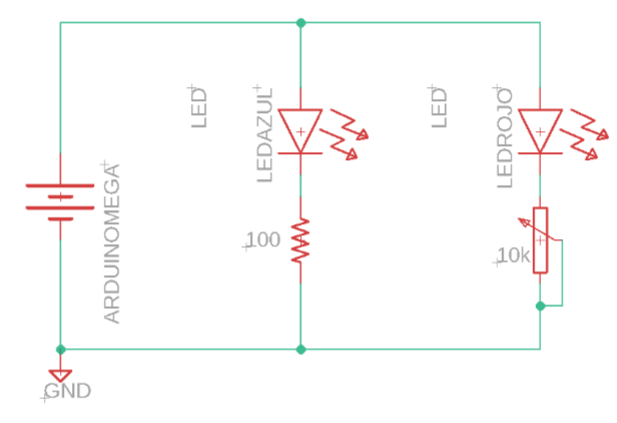
\includegraphics[width=0.50\textwidth]{./img/Circuito-potenciometro.png}
    \caption{Circuito base con potenciometro}
    \label{fig:simulacion_esquema}
\end{figure}

A través de la implementación pudimos entender su funcionamiento y determinar lo siguiente:
\begin{itemize}
    \item El LED azul estará siempre prendido una vez inicie el flujo de corriente, debido a que este se encuentra conectado, en serie, con una resistencia de 100 ohmios, permitiendo el flujo de corriente hacia tierra.
    \item El LED rojo también se encenderá si el pin del Arduino esta en estado alto, sin embargo, su intensidad de brillo dependerá del valor ajustado en el potenciómetro de 10k ohmios
    \item Al ajustar la perilla del potenciómetro se modifica la resistencia en el circuito, lo que cambia la cantidad de corriente que fluye a través del LED. Si disminuyes la resistencia, el LED rojo brillará con mayor intensidad porque circula más corriente, en cambio, si aumentas la resistencia, el brillo del LED disminuirá hasta apagarse si se llega al minimo
    \item Si la fuente de alimentación del Arduino la cambiamos de 5 a 3.3, ambos LEDs podrían verse afectados. En primer lugar, el LED azul no se enciende debido a que estos requieren un voltaje de mínimo 3V y si sumamos la resistencia se pierde mucha corriente ocasionando esto. Por otro lado, el LED rojo si se sigue encendiendo pero con menor brillo, ya que hay menos voltaje y corriente disponibles, especialmente si el potenciómetro esta ajustado a un valor alto.
\end{itemize}

\begin{figure}[H]
    \centering
    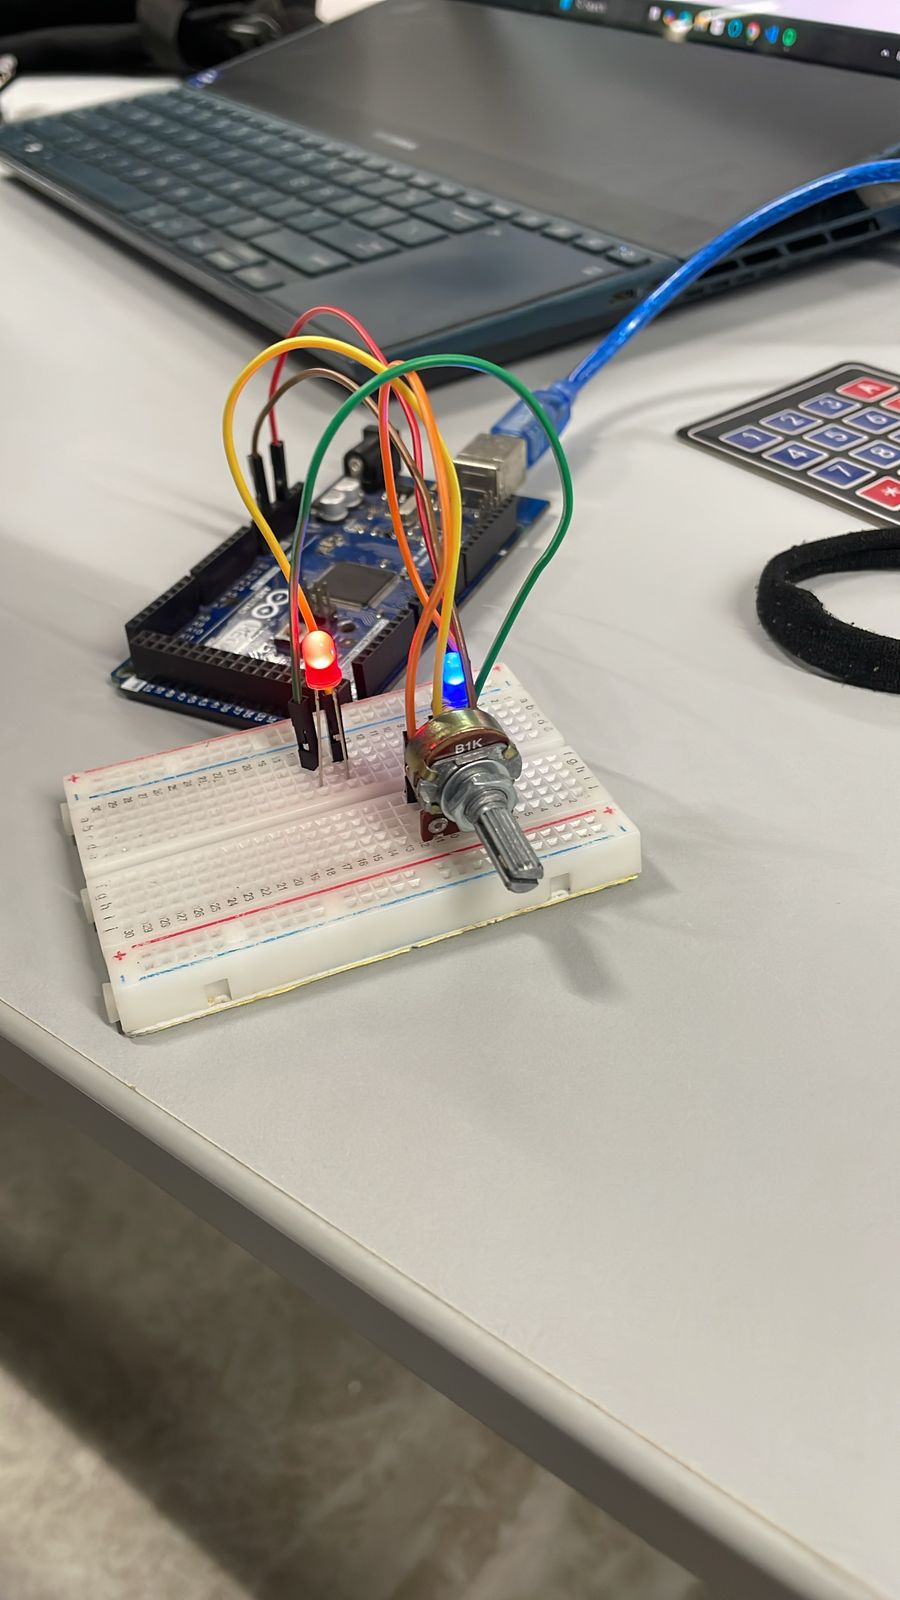
\includegraphics[width=0.50\textwidth]{./img/chkp-3-4-2.jpeg}
    \caption{Implementación LED-Potenciometro 2}
    \label{fig:simulacion_esquema}
\end{figure}

\begin{figure}[H]
    \centering
    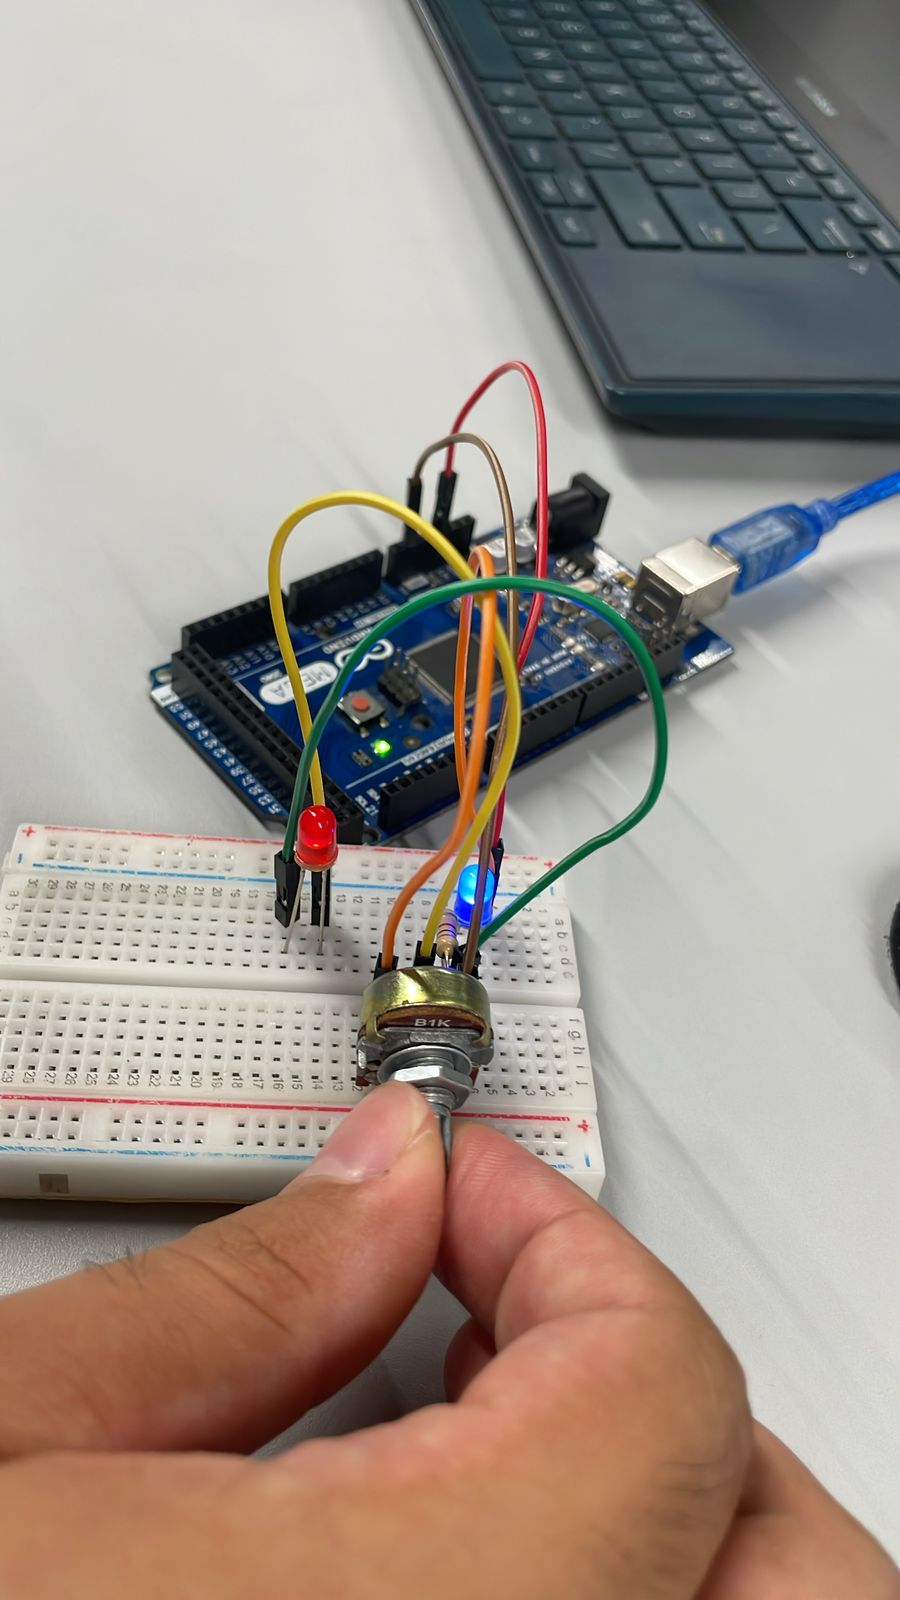
\includegraphics[width=0.50\textwidth]{./img/chkp-3-4-1.jpeg}
    \caption{Implementación LED-Potenciometro 2}
    \label{fig:simulacion_esquema}
\end{figure}

\subsection{Checkpoint 5: Uso de un botón}

\begin{figure}[H]
    \centering
    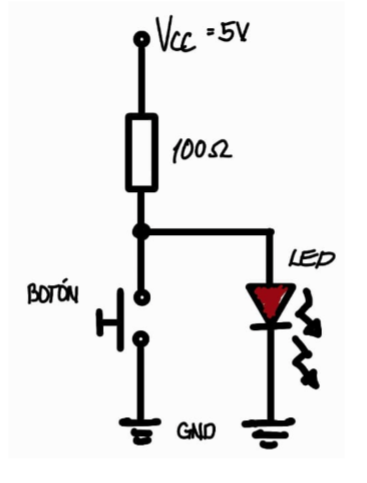
\includegraphics[width=0.50\textwidth]{./img/Circuito-boton.png}
    \caption{Circuito base con boton}
    \label{fig:simulacion_esquema}
\end{figure}

\begin{figure}[H]
    \centering
    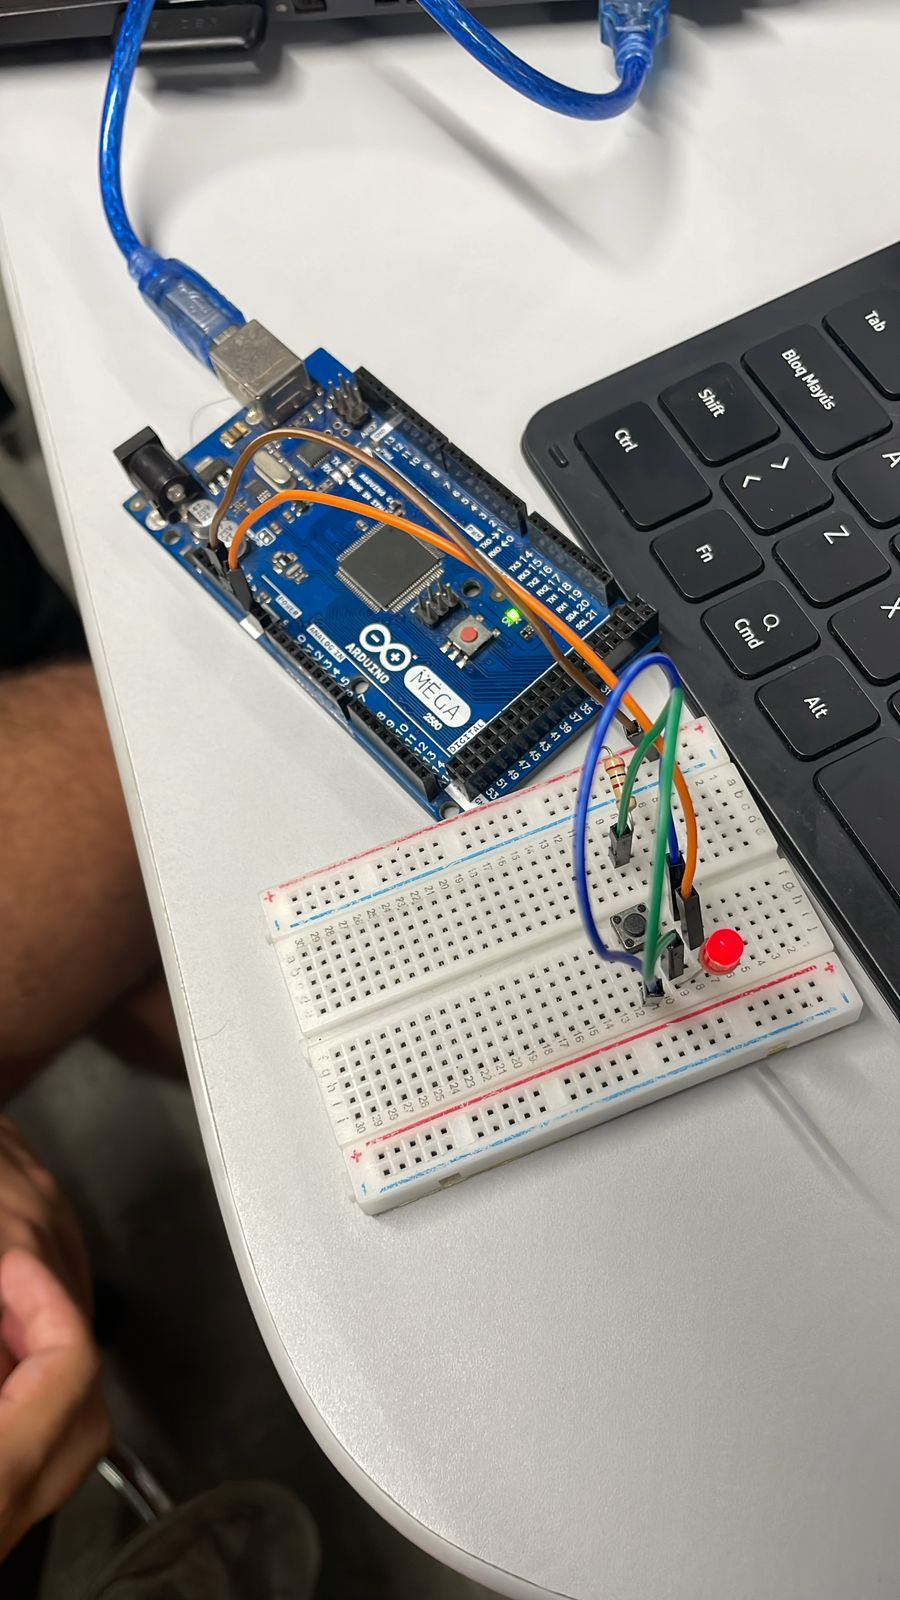
\includegraphics[width=0.50\textwidth]{./img/chkp-3-5-1.jpeg}
    \caption{Implementación del circuito con boton}
    \label{fig:simulacion_esquema}
\end{figure}

\subsection{Checkpoint 6: LEDs secuenciales}

En este ejercicio se propone el diseño, simulación e implementación de un sistema que utiliza cuatro diodos LED (rojo, azul, verde y amarillo) que se encienden de manera secuencial en un orden predefinido. Además, se incluye un botón que permite cambiar la dirección de la secuencia de encendido de los LEDs de forma instantánea, sin necesidad de completar el ciclo actual. Este sistema busca reforzar los conceptos básicos de control de hardware mediante Arduino, incluyendo el uso de salidas digitales y la lectura de entradas digitales para modificar el comportamiento del sistema.

El funcionamiento del sistema se puede dividir en dos modos: 
\begin{itemize}
    \item \textbf{Modo normal (sin presionar el botón):} los LEDs se encienden en el orden rojo → azul → verde → amarillo.
    \item \textbf{Modo inverso (botón presionado):} los LEDs se encienden en el orden amarillo → verde → azul → rojo.
\end{itemize}

La transición entre modos se realiza al detectar un cambio en el estado del botón, y la dirección del encendido cambia de inmediato, lo cual se controla mediante una variable lógica \texttt{flag}.

\begin{figure}[H]
    \centering
    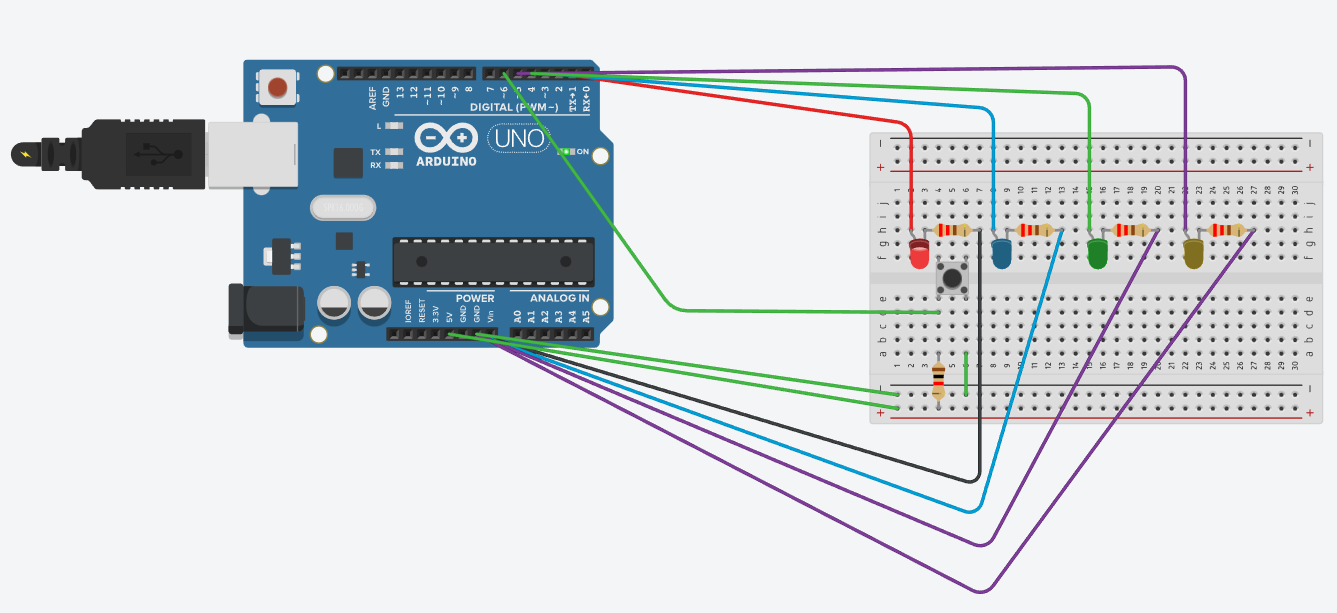
\includegraphics[width=0.85\textwidth]{./img/ckpt_6_0.png}
    \caption{Simulación Tinkercad LEDs secuenciales}
    \label{fig:leds_secuenciales}
\end{figure}

El código mostrado a continuación permite gestionar esta lógica. Cada vez que se ejecuta el bucle \texttt{loop()}, se verifica el estado del botón. Si está presionado, se invierte la dirección de la secuencia. Luego, se incrementa la variable \texttt{color}, y se decide cuál LED encender según el valor de \texttt{color \% 4} y la dirección actual (\texttt{flag}). Al finalizar, se enciende el LED correspondiente durante un segundo y luego se apaga.


\begin{lstlisting}[style=cppstyle, caption={Código en C++ para el control de LEDs secuenciales.}, label={code:leds_secuenciales}]
// C++ code
int actual = 0, color = 0;
bool flag = 1;

void setup()
{
    pinMode(LED_BUILTIN, OUTPUT);
    pinMode(0, OUTPUT);
    pinMode(6, INPUT);
    pinMode(5, OUTPUT);
    pinMode(2, OUTPUT);
    pinMode(3, OUTPUT);
    pinMode(4, OUTPUT);
    Serial.begin(9600);
}

void loop()
{ 
    int buttonState = digitalRead(6);
    Serial.println(digitalRead(6));
    if (buttonState == LOW) flag = !flag;
    color += 1;
    if (flag)
    {
        if (color % 4 == 1) actual = 2;
        if (color % 4 == 2) actual = 3;
        if (color % 4 == 3) actual = 4;
        if (color % 4 == 0) actual = 5;
    } 
    else 
    {
        if (color % 4 == 1) actual = 5;
        if (color % 4 == 2) actual = 4;
        if (color % 4 == 3) actual = 3;
        if (color % 4 == 0) actual = 2;
    }
    digitalWrite(actual, HIGH);
    delay(1000);
    digitalWrite(actual, LOW);
}
\end{lstlisting}

Para facilitar la comprensión del algoritmo y su lógica de decisión, se elaboró el siguiente diagrama de flujo. Este representa gráficamente la secuencia de decisiones y acciones que se ejecutan en el ciclo principal del programa. En él se observa cómo se lee el estado del botón, se actualiza el contador y se determina el LED que debe encenderse, de acuerdo con la dirección actual.

\begin{figure}[H]
    \centering
    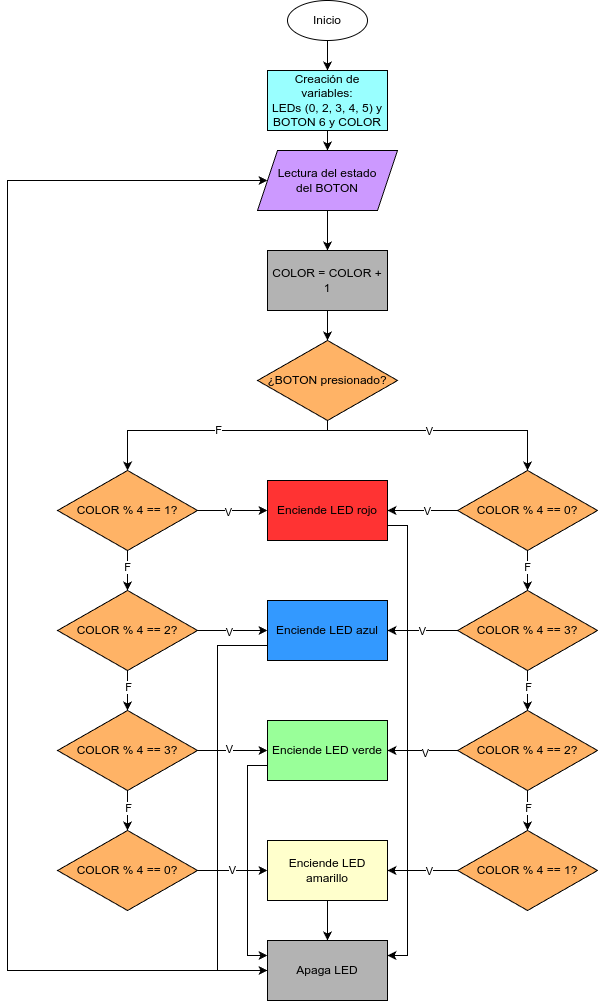
\includegraphics[width=0.6\textwidth]{./img/ckpt_6_1.png}
    \caption{Simulación Tinkercad LEDs secuenciales}
    \label{fig:leds_secuenciales_flowchart}
\end{figure}

\subsection{Checkpoint 7: Semáforo}

\section{Conclusiones}

\bibliographystyle{plain}
\bibliography{bibliografia}

\end{document}

% https://tug.ctan.org/info/undergradmath/undergradmath.pdf
